\section{Background \& Methodology}
\label{sec:background}

%Container-based virtualization (such as Linux Containers~\cite{LXC}) has
%emerged as a lightweight alternative to full virtualization.
%%
%Compared to Virtual Machines (\eg VMware~\cite{VMware} or Xen~\cite{xen}),
%containers work at the operating system level.
%%
%Containers share the same kernel which improves startup times and significantly
%reduces the storage and memory overhead ~\cite{ContainerVirtualization}.

%\subsection{Docker}

Docker~\cite{docker} is a popular container-based virtualization technology
that extends LXC with higher level APIs and additional functionality.
%
It automates the deployment of applications inside Linux containers, and
provides the capability to efficiently package an application with its runtime
dependencies in a container image~\cite{slacker}.



\begin{figure}
	\centering
	% Requires \usepackage{graphicx}
	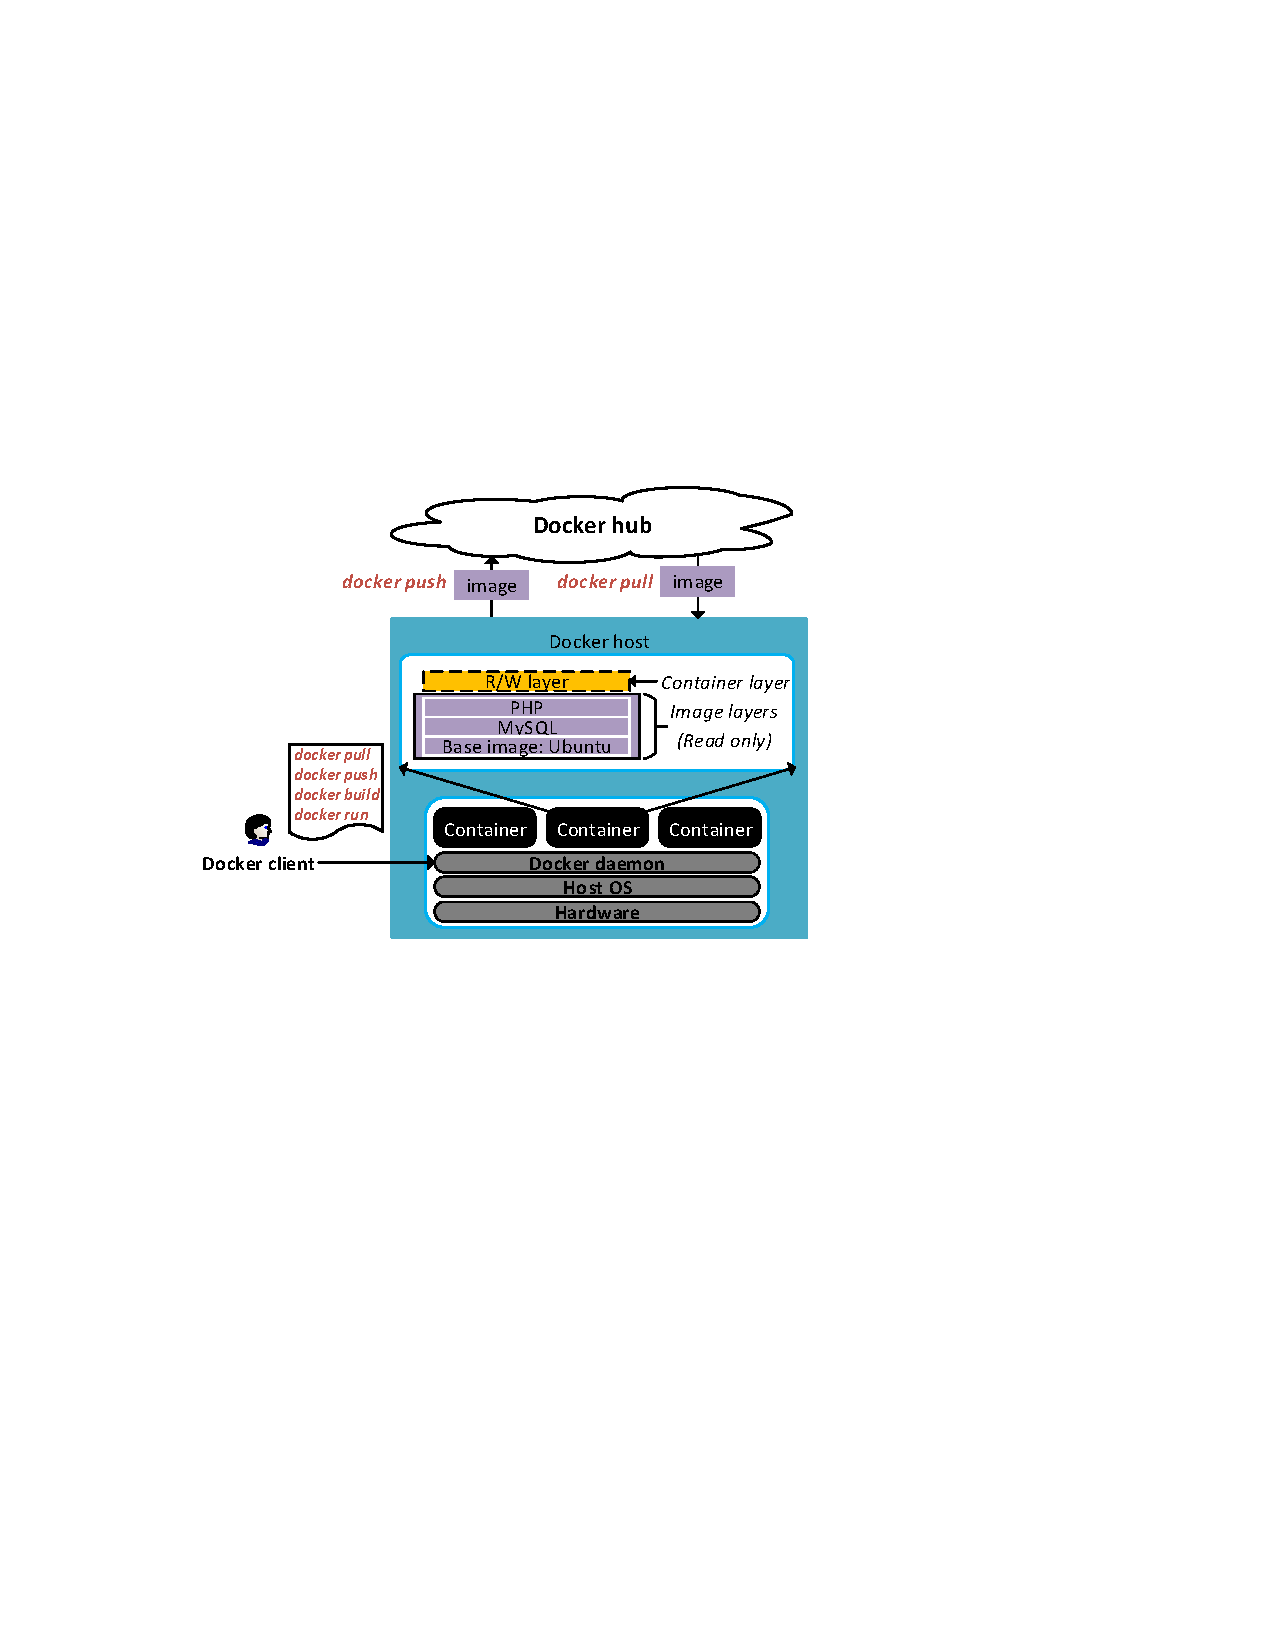
\includegraphics[width=0.5\textwidth]{graphs/fig-docker-architecture}
	\caption{Docker ecosystem
%	\lrcomment{We need to update the figure to capture
%	all the main interactions between the components and remove some unneeded
%	detail, \eg official and unofficial repositories\nancomment{addressed}}
	}
	\label{fig-docker-architecture}
\end{figure}

As shown in Figure~\ref{fig-docker-architecture}, the Docker setup consists of
several components.
%
Users interact with Docker via the Docker \emph{client}, which sends commands
to the Docker \emph{daemon}.
%
The daemon is responsible for \emph{running} containers from locally available
images.
%
Additionally, the daemon supports \emph{building} new images and \emph{pushing}
them to a Docker \emph{registry}.
%
In case a user wants to launch a container from an image that is not available
locally, the daemon will \emph{pull} the required image from the registry.

\subsection{Docker images and layers}
\label{sec-image-layers}

At the center of Docker is the concept of container images for packaging,
distributing, and running applications.
%
Docker images consist of a series of individual \emph{layers}.
%
A layer contains a subset of the files in the image and often represents a
specific component/dependency of the image, \eg a shared library.
%
This modular design allows layers to be shared between two or more images if
both images depend on the same component.

Image layers are read-only.
%
When users start a container via {\tt docker run}, Docker creates a new
writable layer on top of the underlying read-only layers as shown in
Figure~\ref{fig-docker-architecture}.
%
Any changes made to files in the image will be reflected inside the writable
layer via a copy-on-write mechanism.
%
This leaves layers unmodified throughout the lifetime of a container and
enables layer sharing between multiple containers spawned from the same or
different images.
%
Docker supports multiple storage drivers, \eg Aufs and Btrfs, which efficiently
combine read-only and writable layers in a single
namespace~\cite{docker-driver-eval}.
%
%The writable layers are deleted when the container is deleted.

%Image is represented by a \emph{manifest} which describes the various
%constituents of a Docker image, such as the target hardware platform and
%environment settings.
%%
%Moreover, the manifest contains a list of layer digests for all layers required
%by the image.


\subsection{Docker registry}
\label{sec:docker-registry}

The Docker registry is a platform for storing and sharing container images.
%
It stores images in \emph{repositories}, each containing different versions of
the same image.
%
Image layers are stored as \textbf{compressed archival files} and image
manifests as JSON-based files.
%
%Docker Hub is one of the most popular public registries, supporting both
%public and private repositories, via which users can upload, search, and
%download images~\cite{docker-hub}.
%
%In Docker Hub, the user repositories are namespaced by user name, i.e.,
%``$\langle username\rangle/\langle repository name \rangle$", while the
%official repositories, which are directly provided by Docker Inc. and partners
%are called ``$\langle repository name \rangle$".

Modern Docker registry identifies and addresses a layer with a digest that is
computed based on the layer's content (e.g., SHA-256).
%
This allows registry to store only one instance of a layer even if multiple
users accidentally built identical layers.
%
Notice, however, that even if a single file in two otherwise identical layers
differs, the two layers are treated as completely different and stored in their
entirety.
